\clearpage

\section{Oxford Nanopore Technologies: cDNA Sequencing}
\label{sec:ONT_cDNA_Sequencing}
%https://www.nature.com/articles/s41587-020-0731-9

\subsection{Introduction}
Following the success of PacBio's SMRT for generating long sequencing reads in real-time (reviewed in \cref{tab: longread_isoseqstudies}), Oxford Nanopore Technologies (ONT) introduced an alternative long-read, single-molecule sequencing technology with the commercial release of the MinION in 2014. In contrast to all existing sequencing applications which rely on a "sequencing-by-synthesis" approach (including PacBio's SMRT sequencing), ONT technology pioneered the approach of directly reading a single DNA strand using a protein nanopore rather than by measuring incorporation events on the template strand\cite{Jain2015} (\cref{fig:ONT_Mechanism}\textbf{A}). Partly owing to the relatively lower cost and portability of ONT technology, nanopore sequencing has been widely used for transcriptome profiling (reviewed in \cref{tab: longread_ontstudies}), 
with theoretically no upper limit to read length \cite{Loman2015} (the longest read to date is over 150kb), and with no bias towards length or GC content \cite{Oikonomopoulos2016, Weirather2017}.


\subsubsection{Mechanism}
The MinION is a hand-held portable USB-powered device. At its centre is a flow cell that contains a sensor array, which houses a total of 2048 individual nanopores that are controlled in four groups of 512 channels; this allows up to 512 independent DNA molecules to be sequenced simultaneously\cite{Jain2015}. As a voltage is applied across the nanopore, the single-stranded DNA molecules translocate through the nanopore and subsequently interrupt the current in a nucleotide-dependent manner, generating a unique signal of electric current perturbations that acts as proxy of the underlying nucleotide sequence (\cref{fig:ONT_Mechanism}\textbf{A}). 

Successful nanopore sequencing requires the efficient capture and threading of ssDNA into the pore, followed by the ability to identify individual DNA bases in a time-resolved manner. This was achieved through several key innovations\cite{Bayley2015} 
\begin{enumerate}
	\item Generation of an internal positive charge within the protein nanopore to induce capture of negatively-charged DNA. Each nanopore is embedded into an electrical resistant membrane that is immersed in an electrolyte solution.
	\item Discovery and usage of biological pore proteins from the \textit{Staphylococcus aureus} \textit{α}HL\cite{N2005} pore, the \textit{Mycobacterium smegmatis} MspA pore\cite{Manrao2011} to the current \textit{Escherichia coli} CsgG pore. The modified CsgG pore contains a short and narrow channel constriction site, enabling detection of distinct ionic currents at a single-nucleotide resolution. 
	\item Ratcheting the DNA through the pore for time-resolved base identification with a processive enzyme (henceforth referred to as a motor protein, \cref{fig:ONT_Mechanism}\textbf{A,B}), which facilitates DNA movement and reduces the translocation speed of the molecule for improved signal (average speed of 450bp/s)\cite{Rang2018}. This processive enzyme is ligated to the 5'end of both strands during library preparation.   
\end{enumerate}

\begin{figure}[]
	\centering
	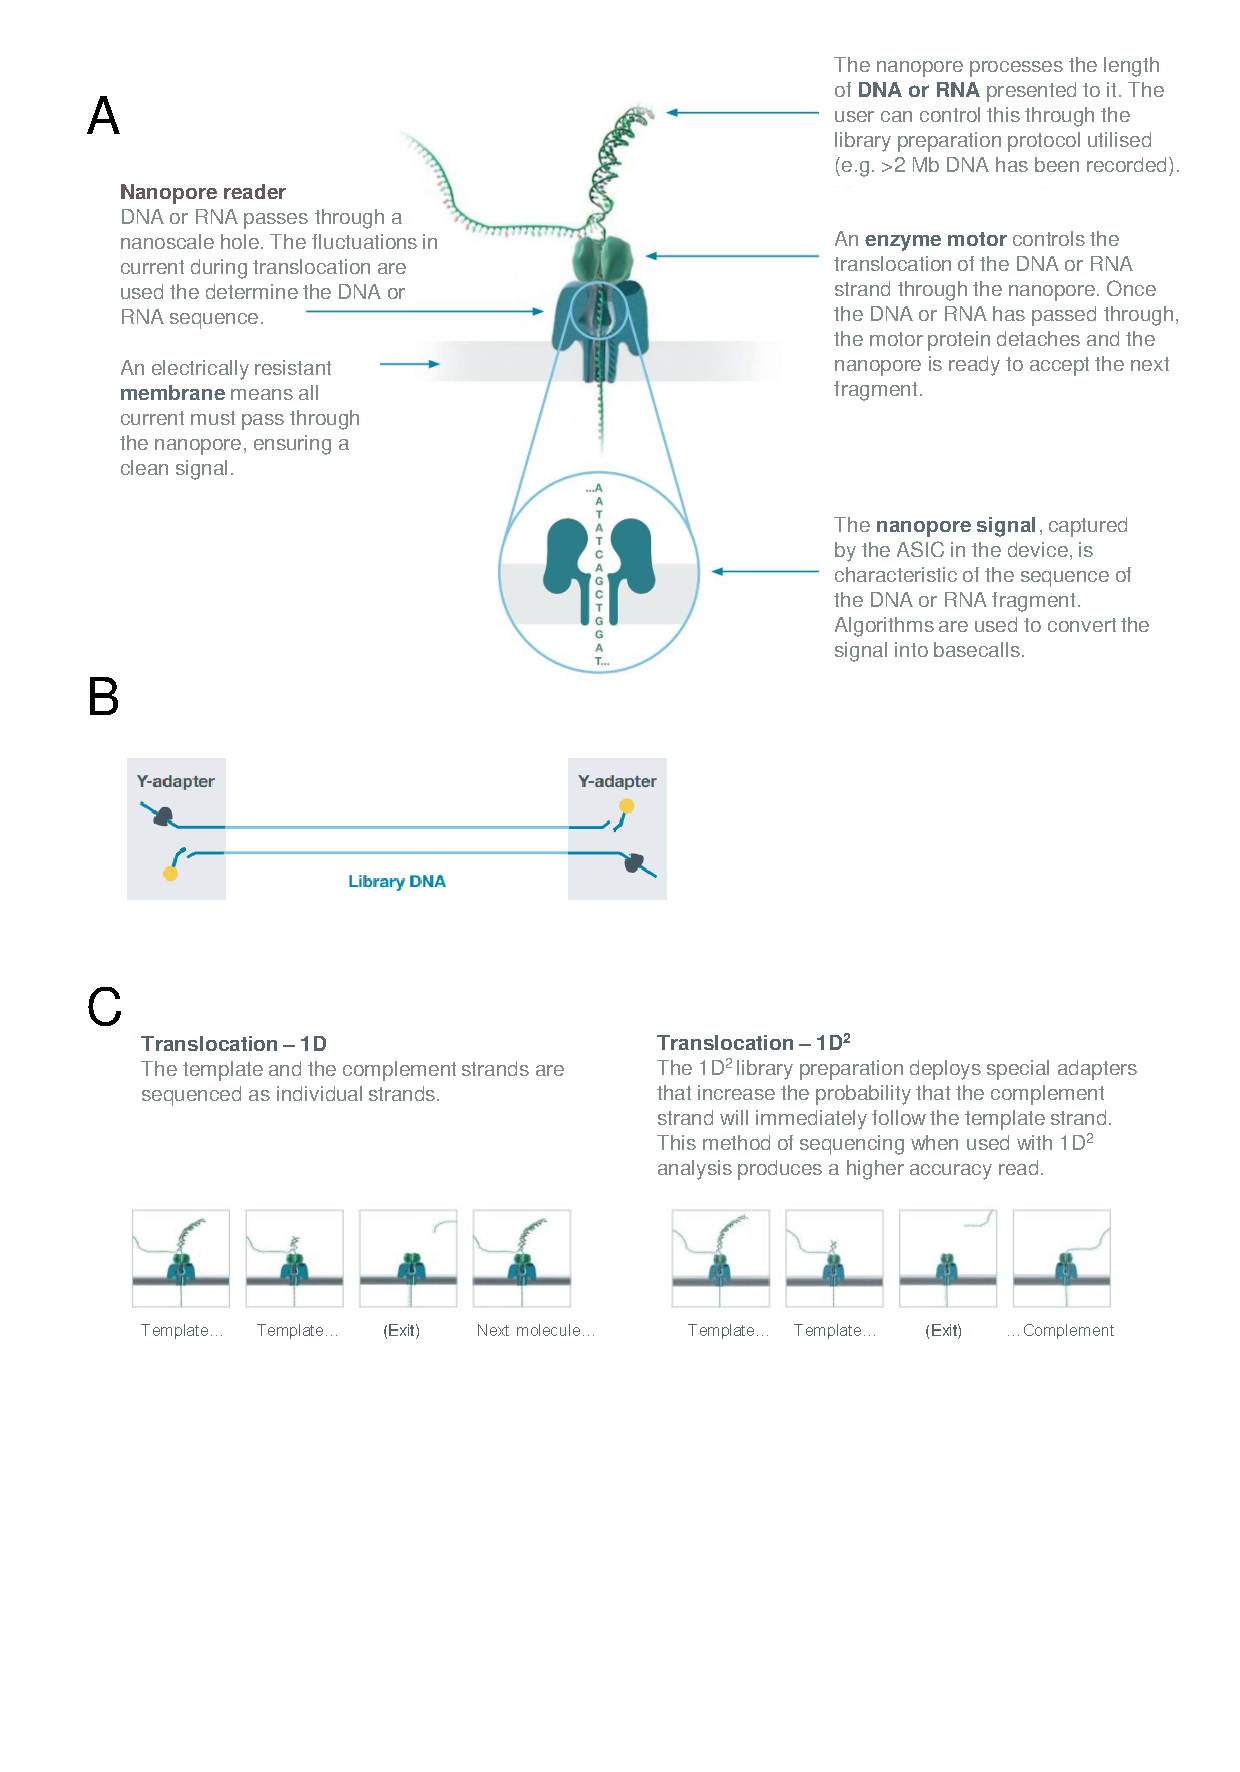
\includegraphics[page=1,trim={0 6cm 0 0 },clip, scale = 0.8]{Figures/ProjectDevelopment_FiguresONT}
	\captionsetup{width=0.95\textwidth}
	\caption[ONT's Nanopore cDNA Sequencing]%
	{\textbf{ONT's Nanopore cDNA Sequencing.}\textbf{A)} Oxford Nanopore Technologies pioneered the development of sequencing DNA through a biological nanopore. The translocation of the sequence, controlled by the enzyme motor protein, causes nucleotide-sensitive perturbations in the electric current. \textbf{B)} The structure of the library DNA with ligation of the sequencing adapter, containing the motor protein (brown circle), to the template and complementary strand. \textbf{C)} Two sequencing translocation modes are currently offered, generating either 1D or 1D\textsuperscript{2} reads. Figures are taken from Oxford Nanopore Product Brochure July 2018.}
	\label{fig:ONT_Mechanism}
\end{figure}

\clearpage
\subsection{Lab Workflow}
\label{chap:ont_labpipeline}
This section describes the library preparation for ONT cDNA sequencing experiments used in \textbf{Chapter 6} for the targeted transcriptome profiling of AD genes in the mouse cortex. At the time of my PhD research, the ONT technology was significantly less advanced that the PacBio technology with only basic protocols. Nanopore sequencing was therefore conducted on a subset of mouse samples as a source of validation and technology comparison using methods optimised during my research. 

For a fairer and more direct comparison, all steps prior to the ONT library preparation were adopted from the Iso-Seq protocol, including the conversion of RNA to cDNA using the SMARTer PCR cDNA synthesis (\cref{section:ch2_cDNA_synthesis_explanation}), large scale DNA amplification using the GXL DNA Polymerase and target enrichment with hybridisation-based capture (workflow is depicted in \cref{fig:ONT_TargetedProtocol}). Consequently, nanopore reads are generated with the same cDNA primers and barcode sequences as Iso-Seq reads (refer to \cref{tab:barcode_primers} for sequences). Post cDNA synthesis and amplification, the ONT library preparation is broadly similar to the Iso-Seq library preparation (also outlined in \cref{fig:ONT_TargetedProtocol}), with the exception that the motor enzyme is pre-bound to the adapters in ONT reads whereas the polymerase is only loaded after adapter ligation in Iso-Seq.  

\begin{figure}[]
	\centering
	\includegraphics[page=7,trim={0 6cm 0 0 },clip, scale = 0.7]{Figures/ProjectDevelopment_FiguresONT}
	\captionsetup{width=0.95\textwidth}
	\caption[ONT and Iso-Seq Lab workflow for targeted transcriptome profiling]%
	{\textbf{ONT and Iso-Seq Lab workflow for targeted transcriptome profiling.} Shown is a flow diagram of the ONT lab workflow in parallel with the Iso-Seq lab workflow for a fair and direct comparison of targeted transcriptome profiling. RNA was barcoded (denoted by the orange and purple star), converted to cDNA using SMARTer PCR cDNA synthesis kit. Amplified and purified cDNA was then pooled in equimolar quantities across multiple fractions and samples, followed by with target gene enrichment using the hybridisation-based capture (IDT), respective library preparation and sequencing.}
	\label{fig:ONT_TargetedProtocol}
\end{figure}


\subsubsection{ONT MinION Library Preparation}
\label{sec: ONTlib_preparation}
After obtaining high-quality and full-length cDNA, nanopore library preparation was performed using the SQK-LSK109 1D sequencing by ligation protocol (outlined in \cref{fig:ONT_Protocol}). Library preparation is a relatively simple process; cDNA ends were first repaired and dA-tailed using the NEBNext End Repair/dA-tailing Module, followed by 1X AMPure Bead Purification and adapter ligation. The library was then subjected to a final round of 0.4X AMPure Bead Purification before loading into the ONT MinION for sequencing. The ONT sequencing adapters (depicted in \cref{fig:ONT_Mechanism}\textbf{B}) contained a dT overhang for ligation to the dA-ends of cDNA, the pre-bound motor protein, and a cholesterol moiety which facilitates DNA capture by tethering the molecule to the flow cell's lipid membrane.
%SQB and LB were used with the human samples ran on ONT rather than RBF (Aaron's comment)

\clearpage
\begin{figure}[!h]
	\centering
	\includegraphics[page=3,trim={0 16cm 0 0 },clip, scale = 0.7]{Figures/ProjectDevelopment_FiguresONT}
	\captionsetup{width=0.95\textwidth}
	\caption[ONT library preparation with 1D ligation sequencing kit]%
	{\textbf{ONT library preparation with 1D ligation sequencing kit.} Shown is a flow diagram of the ONT library preparation with the ONT ligation sequencing kit (SQK-LSK109), which primarily involved repairing cDNA ends and dA-tailing followed by ligation of sequencing adaptors. The motor protein and cholesterol moiety are represented by the brown and yellow circle, respectively. Figure is adapted from ONT Nanopore Protocol 1D amplicon/cDNA by Ligation (SQK-LSK109).}
	\label{fig:ONT_Protocol}
\end{figure}


\subsubsection{Priming the Flow Cell and Sequencing}
\label{sec: ONTlib_sequencing}
Nanopore sequencing was performed on the MinION using a Min106D Flow cell, which contains the R9 nanopore (as shown in \cref{fig:ONT_advances}). Prior to sequencing, the flow cells were tested for the total number of functional pores present and were only used if >800 pores were available (as recommended by ONT). The flow cell was subsequently primed for sequencing with a "Running buffer with fuel mix" (RBF), which contained the substrate cofactor essential for efficient motor protein activity (i.e. ATP for the ATPase activity of the helicase component of the translocation motor). The library was then loaded into the MinION with Library Loading Beads (LLB), which are sepharose beads that work on a principle similar to Iso-Seq MagBeads by immobilising the library to the lipid membrane.

% https://community.nanoporetech.com/posts/flo-minxxx-x-rx-x-r
\subsection{Run Performance and Quality Metric}
\label{ONT_performance}
One major drawback of nanopore sequencing is the relatively high error rate compared to short-read (i.e. Illumina) sequencing, which can arise from random and systematic error during sequencing or during translation of the raw electric signal into a DNA sequence (a process known as basecalling)\cite{Rang2018}. The first error is exacerbated by the fact that i) several nucleotides occupy the pore at any given time point, resulting in multiple effects on the signal, and that ii) the signal does not change with translocation of homopolymers (stretches of identical bases).

However, major advances in the basecalling algorithms, the chemistry and nanopore itself have drastically increased the accuracy of single-pass sequencing reads from 60\% \cite{Jain2015}, to 98.3\% (vR.9.4.1 and Bonito) (\cref{fig:ONT_advances}), and more recently at the beginning of 2021, 99\% (Q20+)\cite{OxfordNanoporeTechnologiesplc.2021}. These developments include the ability to sequence the complementary strand immediately after the template strand, thereby attaining a more accurate consensus read (1D\textsuperscript{2}) that increases the accuracy of template reads (1D) alone by 5\%\cite{Rang2018} (\cref{fig:ONT_Mechanism}\textbf{C}), though at the expense of throughput \cite{NanoporeCommunityPosts}. Of note, earlier releases of nanopore sequencing offered 2D sequencing which involved ligation of both strands with a hairpin adapter, though this has been largely replaced by 1D\textsuperscript{2} sequencing. However, the error rate still falls slightly short of the 99.9\% achieved by PacBio's CCS reads and short-read platforms, and errors near splice sites can result in spurious alignments and in correct clustering of reads. Other approaches to mimic the PacBio's circular consensus approach have been proposed (i.e. INC-seq \cite{Li2016c} and R2C2 \cite{Volden2018}), with accuracy approaching 97.5\%. However, such methods are laborious and not commonly used.  

\begin{figure}[h]
	\centering
	\includegraphics[page=2,trim={0 19cm 0 0},clip, scale = 0.8]{Figures/ProjectDevelopment_FiguresONT}
	\captionsetup{width=0.95\textwidth}
	\caption[Significant advances in ONT nanopore sequencing read accuracy]%
	{\textbf{Significant advances in ONT nanopore sequencing read accuracy.} Optimisation in the structure of nanopores (chemistry updates) and development in basecalling algorithms have led to drastic improvements in read accuracy. The R7 and R9 nanopore series is based on the MspA and CsgG protein, respectively. Of note, the figure does not include the latest chemistry (1D\textsuperscript{2}) or nanopore development (R.10.4, this involves a longer barrel and two pinch points to provide better resolution of homo-polymer sequences). Figure is taken from Rang et al.(2018)\cite{Rang2018}}
	\label{fig:ONT_advances}
\end{figure}

\newpage
In contrast to PacBio SMRT sequencing, real-time feedback and progress of the nanopore sequencing run are provided with information given on the run statistics (i.e. the total number of reads generated at any time) and the channel states over time. The channel state is an indication of the pore occupancy and is classified as being either i) sequencing (active with current DNA translocation), ii) pore (active but without DNA translocation), iii) recovering, iv) inactive and v) unclassified (channels are divided into 4 groups and used sequentially to maximise throughput, and unclassified channels are those that not currently used). The duty time plot provides a good assessment of the current performance of the run, and an early indication whether to continue or stop the run (examples of successful and suboptimal runs are given in \cref{fig:ONTPoreOccupancy}). 

\begin{figure}[]
	\centering
	\includegraphics[page=6,trim={0 14cm 0 0 },clip, scale = 0.8]{Figures/ProjectDevelopment_FiguresONT}
	\captionsetup{width=0.95\textwidth}
	\caption[Examples of successful and suboptimal ONT nanopore sequencing runs]%
	{\textbf{Examples of successful and suboptimal ONT nanopore sequencing runs.} Shown are duty time plots from \textbf{A)} a good quality run indicated by the majority of pores in the "sequencing" state (bright green), \textbf{B)} a suboptimal run with channels being blocked as indicated by an accumulation of pores in the "recovering" state (dark blue), \textbf{C)} a suboptimal run with low pore occupancy as indicated by the high ratio of "pore" (dark green) to "sequencing" state, and \textbf{D)} a suboptimal run with flow cell failure indicated by the majority of pores in "inactive state" (light blue). 
	\\ \\
	Channel blocking typically occurs when there are contaminants in the library. Conversely, low pore occupancy suggests insufficient loading material or poor library preparation (poor ligation reaction). Flow cell failure indicate damaged channel or membranes, which can be caused by multiple factors (air bubbles, osmotic imbalance, presence of detergents in library). Figures are taken from Wellcome Trust Advanced Course: RNA Transcriptomics (2018). Channel states are classified as sequencing (bright green), pore (dark green), recovering (dark blue), inactive (light blue) and unclassified (grey).}
	\label{fig:ONTPoreOccupancy}
\end{figure}

\clearpage
\subsection{Bioinformatics Pipeline}
\label{section:ont_bioinformatics}
This section describes the bioinformatic pipeline for processing and analysing ONT cDNA sequencing data generated on the MinION following ONT library preparation (\cref{ch: targeted_transcriptome}). 

Unlike the Iso-Seq bioinformatics pipeline which was largely established by PacBio (described in \cref{section:isoseq_bioinformatics} and outlined in \cref{fig:isoseq_bioinformatics_Pipeline}), the bioinformatics pipeline for processing ONT raw reads was less defined and streamlined when I undertook this work. While significant improvements in bioinformatic tools have been released by ONT over recent years, many of the new tools were only applicable to sequencing data generated from ONT-specific protocols and primers. Given that the ONT dataset in this thesis was generated using the same primers and barcodes as the Iso-Seq dataset (illustrated in \cref{fig:ONT_TargetedProtocol}), the initial stage of the bioinformatics pipeline was adapted from a protocol from the "Wellcome Trust Advanced Course: RNA Transcriptomics (2018)" (provided by J.Ragoussis and henceforth referred to as WTAC), which I attended during my PhD, and refined using ERCC control oligos as a benchmark. Many of the downstream tools initially developed for Iso-Seq were then similarly applied for the latter stages of the ONT bioinformatics pipeline, with the exception of the use of \textit{TALON} in place of \textit{Cupcake} for collapsing transcripts. Consequently, the bioinformatics pipeline for processing and analysing the ONT targeted cDNA sequencing data is broadly similar to the pipeline previously tailored for the Iso-Seq targeted dataset (refer to \cref{fig:ONT_PacBio_bioinformatics} for comparison). 

\begingroup
\parindent=0em
\etocsettocstyle{\rule{\linewidth}{\tocrulewidth}\vskip0.5\baselineskip}{\rule{\linewidth}{\tocrulewidth}}
\etocsetnexttocdepth{5}
\localtableofcontents 
\endgroup

\begin{figure}[htp]
	\centering
	\includegraphics[page=15,trim={0cm 6cm 0cm 0cm},clip,scale = 0.8]{Figures/ProjectDevelopment_Figures}
	\captionsetup{width=0.95\textwidth,singlelinecheck=off}
	\caption[Comparison of the bioinformatics pipeline for processing PacBio Iso-Seq and ONT 1D-reads]%
	{\textbf{Comparison of the bioinformatics pipeline for processing PacBio Iso-Seq and ONT 1D-reads.} Shown is a side-by-side comparison of the bioinformatics pipeline used to process PacBio Iso-Seq and ONT 1D-reads from initial processing of raw reads, alignment to reference genome with \textit{Minimap2}, to collapse of reads to transcripts and final isoform annotation with \textit{SQANTI}. The bioinformatic pipelines adopted are largely similar between Iso-Seq and ONT with the difference primarily in the initial processing of raw reads; raw Iso-Seq reads were processed with the PacBio bioinformatics suite (\textit{Iso-Seq3}) whereas raw ONT reads were processed using various community-based packages.   
	}
	\label{fig:ONT_PacBio_bioinformatics}
\end{figure}

\clearpage
\subsubsection{Quality Control of Run, Base-calling and Filtering of Base-called Reads}
The performance of each nanopore sequencing run was assessed using \textit{PycoQC}\cite{Leger2019} and the official Nanopore QC tutorial\cite{ONT2019NanoporeQC} by evaluating i) the number of active pores during the run, ii) the number of reads generated over time, and iii) the length and quality score distribution of basecalled reads. ONT raw reads were then basecalled using \textit{Guppy}, the latest released ONT basecaller that converts the raw electrical signal to DNA sequence and is superior to other available basecallers with higher read accuracy and faster basecalling\cite{Wick2019}. Basecalled reads with read quality score < 7 (recommended by ONT) were discarded using \textit{Nanofilt}\cite{DeCoster2018} (v2.3.0) with default parameters.

\subsubsection{Removing of Nanopore and cDNA sequencing adapters}
cDNA primer sequences and nanopore sequencing adaptors were removed to prevent spurious alignment using \textit{Porechop}\cite{Wick2017} (v0.2.4). Under recommended parameters (--end\_size 100, --adapter\_threshold 90, --end\_threshold 75, --min\_trim\_size 15, --discard\_middle, --extra\_end\_trim 1), a window of 100 nucleotides from the end of each read was searched for a set of adaptors, which must have a minimum 90\% identity to be considered present for trimming and a minimum 75\% at the end of the reads; alignments smaller than 15bp or those found within the middle of the reads were considered chimeric and discarded. 

Notably, \textit{Porechop} has been unsupported since 2018 and has been largely replaced by the ONT official tool, \textit{Pychopper}\cite{OxfordNanoporePychopper}. Despite being recommended for ONT-specific barcode demultiplexing, \textit{Pychopper} failed to differentiate and orientate reads from the plus and minus strand without unique sequences, rendering all the ONT reads in the targeted dataset as being "unclassified". Given that the ONT cDNA reads were generated using the SMARTer cDNA synthesis kit (Clontech) (described in \cref{section:ch2_cDNA_synthesis_explanation}, depicted in \cref{fig:ONT_cdnatemplate}\textbf{A}), the 5’ end of the plus and minus strands are reverse complements of each other with a few nucleotide differences (plus strand ends with ATGGG whereas the minus strand ends with polyT, \cref{fig:ONT_cdnatemplate}\textbf{B}). Conversely, \textit{Porechop} was able to differentiate the strand orientation with input of the unique set of adaptors that includes the cDNA primers, ONT adaptors and corresponding polyA/T tail (provided in \cref{tab:ont_barcode}). Sample demultiplexing was also performed by including the 16bp barcode sequence, and reads were assigned to the sample with the highest identity. 

Trimmed reads with adaptors present at both ends were retained, and reads corresponding to the minus strand were reverse complemented. Using \textit{Cutadapt}\cite{Martin2011} (v2.9, -a "A{40}"), the polyA sequence was then trimmed 40 nucleotides from the 3'end.

\begin{figure}[ht]
	\begin{center}
		\includegraphics[page=22,trim={0cm 18cm 0cm 1cm},clip, scale = 0.7]{Figures/ProjectDevelopment_Figures.pdf}
	\end{center}
	\captionsetup{width=0.95\textwidth}
	\caption[Structure of ONT cDNA template]%
	{\textbf{Structure of ONT cDNA template.} Shown is the \textbf{A)} final structure of the cDNA molecules for ONT sequencing, after cDNA synthesis and adaptor ligation, and the corresponding differentiating start and end sequence for the plus and minus strands \textbf{B)} and with just the adaptor sequences for comparison between the different read strands. The original cDNA molecules are outlined in purple and green, and the ONT boxes indicate the position of the ONT sequencing adaptors. The barcode location of sample demultiplexing is indicated in red (see \cref{tab:barcode_primers} and \cref{tab:ont_barcode} for barcode sequences). 
	\\ 
	\\	
	As illustrated, the barcode is only present in the 3'end of the plus strand and 5'end of the minus strand, as part of the oligo-dT primer during cDNA synthesis (\cref{tab:barcode_primers}). The differing nucleotides between the plus start and the minus start is highlighted in yellow. The brown and orange circle refer to the motor protein and cholesterol moiety, respectively. The start and end of the strand is defined by the 5' and 3' end, respectively. }
	\label{fig:ONT_cdnatemplate}
\end{figure}

\begin{landscape}
	\begin{table}[]
		\centering
		\captionsetup{width=0.95\linewidth}
		\caption[ONT adapter sequences for plus and minus strand of barcoded samples]%
		{\textbf{ONT adapter sequences for plus and minus strand of barcoded samples.} Tabulated are the sequences used in \textit{Porechop} for sample demultiplexing and identifying the plus and minus strands. As depicted in \cref{fig:ONT_cdnatemplate}, only the plus strand end sequences and the minus strand start sequences contain the sample-specific barcode sequence (reverse complementary of one another). BC - Barcode}
		\label{tab:ont_barcode}
		\begin{tabular}{@{}ccccc@{}}
			\toprule
			\multirow{2}{*}{Barcoded  Samples} & \multicolumn{2}{c}{Plus strand} & \multicolumn{2}{c}{Minus strand} \\ \cmidrule(l){2-5} 
			& Start sequence & End sequence & Start sequence & End sequence \\ \midrule
			BC1 & \multirow{10}{*}{\begin{tabular}[c]{@{}c@{}}TTGCTAAG\\ CAGTGGTA\\ TCAACGCA\\ GAGTACAT\\ GGG\end{tabular}} & AAAAAACGCACTCTGATATGTGGCA & CACATATCAGAGTGCGTTTTTT & \multirow{10}{*}{\begin{tabular}[c]{@{}c@{}}CCCATGTAC\\ TCTGCGTTG\\ ATACCACT\\ GCTTAGCAAT\\ ACGTAACT\end{tabular}} \\
			BC2 &  & AAAAAAACTCACAGTCTGTGTGTGCA & ACACACAGACTGTGAGTTTTTTT &  \\
			BC3 &  & AAAAAAACTCTCACGAGATGTGTGCA & ACACATCTCGTGAGAGTTTTTTT &  \\
			BC4 &  & AAAAAAACGCGCGTGTGTGCGTGGCA & CACGCACACACGCGCGTTTTTTT &  \\
			BC5 &  & AAAAAAAACGCGAGAGTCGAGTGGCA & CACTCGACTCTCGCGTTTTTTTT &  \\
			BC6 &  & AAAAAAAACAGCTGATATATATGGCA & CATATATATCAGCTGTTTTTTTT &  \\
			BC7 &  & AAAAAAACACATAGAGATACAGAGCA & TCTGTATCTCTATGTGTTTTTTT &  \\
			BC8 &  & AAAAAAACGCAGCGCTCGACTGTGCA & ACAGTCGAGCGCTGCGTTTTTTT &  \\
			BC9 &  & AAAAAAATCTGTCTCGCGTGTGTGCA & ACACACGCGAGACAGATTTTTTT &  \\ \hline
		\end{tabular}
	\end{table}
\end{landscape}

\subsubsection{Genome Alignment and Transcript Collapse}
Trimmed reads from each sample were then aligned to the reference genome using \textit{Minimap2}\cite{Li2018} (v2.17-r941, parameters: -ax splice) and were processed using \textit{TALON}\cite{Wyman2019} for simultaneous transcript discovery and quantification (depicted in \cref{fig:ONT_Talon}). After trialling various bioinformatic tools, including \textit{TAMA}\cite{Kuo2017} and \textit{FLAIR}\cite{Tang2020} (the results of these comparisons are documented in \textbf{Appendix \ref{ONT_Bioinformatics_appendix}}), we found that \textit{TALON} superseded the other tools for a number of reasons, namely i) it allows reference-based error-correction of ONT reads, which was essential for improving the confidence of splice junctions and recovering rare, novel transcripts, ii) it performs quantification-led filtering of novel transcripts, retaining only transcripts that are reproducibly detected in biological replicates, iii) it generates abundance output filea for each sample (associated FL read count for each transcript), facilitating downstream isoform-level analysis, and vi) it requiree less computing memory and time than other approaches.   


\begin{figure}[htp]
	\centering
	\includegraphics[page=23,trim={0cm 11cm 0cm 2cm},clip,scale = 0.7]{Figures/ProjectDevelopment_Figures}
	\captionsetup{width=0.95\textwidth,singlelinecheck=off}
	\caption[Transcript discovery and quantification of ONT reads using \textit{TALON}]%
	{\textbf{Transcript discovery and quantification of ONT reads using \textit{TALON}.} Shown is a schematic figure of using \textit{TALON} for processing and analysing aligned ONT-derived transcripts. Figure is taken from Wyman et al. (2020)\cite{Wyman2019}  
	}
	\label{fig:ONT_Talon}
\end{figure}